\chapter{Budowa i~działanie systemu GGSS (AK)}
\label{cha:ggss}

% setup
\graphicspath{{3_ggss_introduction/static/}}

% content
Niniejszy rozdział zawiera ważne, z~punktu widzenia przeprowadzonych prac, informacje na temat systemu GGSS. Przedstawione tu opisy dotyczą zagadnień takich jak: wysokopoziomowa architektura systemu, struktura warstwy oprogramowania, opis wykorzystywanych przez system urządzeń oraz omówienie cech charakterystycznych środowiska docelowego. 

\section{Wysokopoziomowa architektura systemu GGSS}
System GGSS składa się z~kilku współpracujących ze sobą elementów, przedstawionych (wraz z~występującymi między nimi interakcjami) na rysunku \ref{fig:high_level_architecture}. Znaczenie poszczególnych komponentów projektu jest następujące:
\begin{itemize}
    \item \textbf{urządzenia (ang. \emph{hardware})} - zestaw urządzeń elektronicznych (m.in. liczniki słomkowe, zasilacze wysokiego napięcia i~multipleksery)
    \item \textbf{oprogramowanie GGSS} - zestaw aplikacji wraz z~otaczającą je infrastrukturą, których zadaniem jest sterowanie urządzeniami wchodzącymi w~skład systemu GGSS oraz przetwarzanie zbieranych za ich pomocą danych
    \item \textbf{pliki konfiguracyjne} - proste pliki tekstowe w~formacie XML (\emph{Extensible Markup Language}) \cite{XML_wikipedia}, zawierające informacje o~oczekiwanym sposobie działania systemu (np. maksymalna możliwa wartość napięcia, jakie może zostać ustawione na każdym z~zasilaczy)
    \item \textbf{pliki wynikowe} - pliki tekstowe zawierające wyniki pomiarów wykonywanych przez system oraz rejestr zdarzeń 
    \item \emph{\textbf{SIMATIC WinCC Open Architecture}} \cite{winccoa} - system typu SCADA (\emph{Supervisory Control And Data Acquisition}) \cite{SCADA_wikipedia}, stanowiący część systemu kontroli detektora ATLAS, pozwalający na obserwację i~kontrolę działania poszczególnych poddetektorów
    \item \emph{\textbf{Distributed Information Management System (DIM)}} \cite{DIMwebsite} - protokół komunikacyjny dla środowisk rozproszonych, oparty o~architekturę klient-serwer, zapewniający komunikację między oprogramowaniem systemu GGSS a~systemem WinCC OA
\end{itemize}

\begin{figure}[H]
\centering
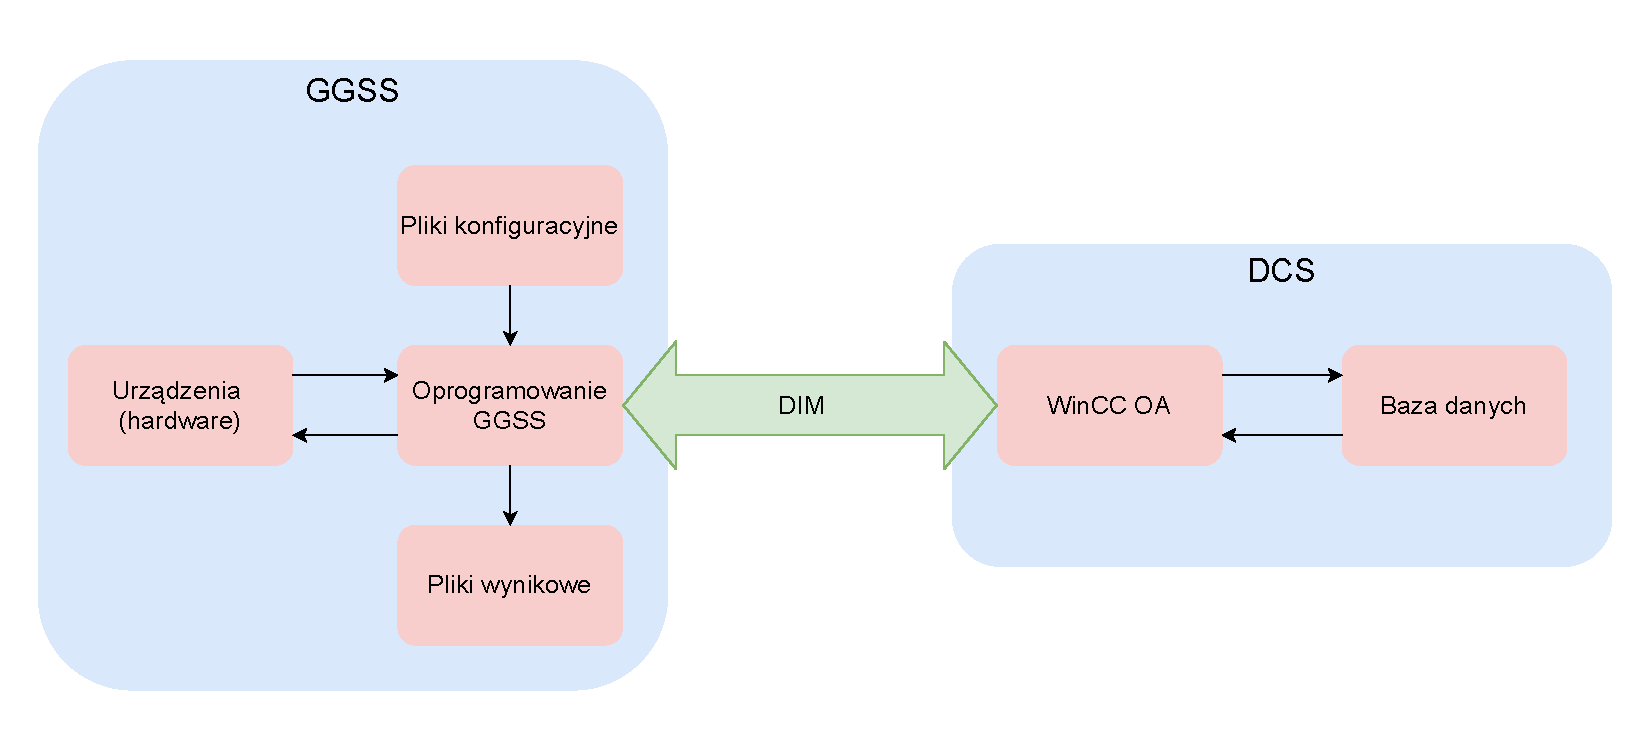
\includegraphics[width=\textwidth]{high_level_architecture.pdf}
\caption{Wysokopoziomowa architektura projektu GGSS. Strzałkami oznaczono przepływ danych pomiędzy poszczególnymi komponentami systemu \cite{GGSS_inz}.}
\label{fig:high_level_architecture}
\end{figure}


Szczegóły działania najważniejszych z~punktu widzenia niniejszej pracy elementów systemu omówione zostaną w~dalszej części tego rozdziału. Znaczna część prac opisanych w~niniejszym manuskrypcie skupiona była na udoskonaleniu warstwy oprogramowania systemu GGSS.


\section{Urządzenia elektroniczne}
Z~punktu widzenia warstwy sprzętowej system GGSS składa się z~zestawu tzw. słomkowych liczników proporcjonalnych, zasilanych za pomocą 4-kanałowych zasilaczy wysokiego napięcia. Sygnały generowane przez liczniki przetwarzane są przez wielokanałowy analizator amplitudy (MCA - \emph{Multi-Channel Analyzer}), natomiast wybór licznika słomkowego używanego do wykonania pomiarów następuje za pomocą 8-kanałowego multipleksera sygnałów analogowych \cite{ZadrozniakInz} \cite{ZadrozniakMgr}. Urządzenia podłączone są do komputera PC, który steruje nimi za pomocą oprogramowania systemu GGSS. W~tabeli \ref{tab:devices} zamieszczone zostało zestawienie informacji na temat wykorzystywanych przez projekt urządzeń. Sposób działania systemu (jego podstawa fizyczna oraz znaczenie przeprowadzanych pomiarów) wykracza poza zakres niniejszej pracy, został natomiast szczegółowo opisany w~pracy \emph{Wybrane zagadnienia związane z~pracą słomkowych liczników proporcjonalnych w~detektorze TRT eksperymentu ATLAS} \cite{mindur_phd}, której autorem jest dr hab. inż. Bartosz Mindur, prof. AGH.

\clearpage

\begin{table*}[htbp]
\centering
\caption{Zestawienie istotnych z~punktu widzenia niniejszej pracy urządzeń wchodzących w~skład systemu GGSS.}
\label{tab:devices}
\begin{tabularx}{\textwidth}{@{}XX@{}}
\toprule
Urządzenie &
Informacje \\
\midrule
4-kanałowy zasilacz wysokiego napięcia & CAEN N1470 \cite{caen} \\
wielokanałowy analizator amplitudy & CAEN N957 \cite{caen} \\
multiplekser sygnałów analogowych & urządzenie autorstwa Pana Pawła Zadrożniaka\\
\bottomrule
\end{tabularx}
\end{table*}


\section{Warstwa oprogramowania}
Poprzez warstwę oprogramowania systemu GGSS autorzy rozumieją zarówno zestaw aplikacji napisanych w~języku C++ (standard 11), jak i~otaczającą je infrastrukturę (pomocnicze skrypty, system budowania, testowania i~tworzenia nowych wydań). 


Trzon warstwy oprogramowania projektu GGSS stanowi aplikacja \emph{ggss-runner}, zawierająca logikę odpowiedzialną za komunikację z~systemem za pomocą protokołu DIM, gromadzenie i~walidację danych oraz sterowanie urządzeniami wchodzącymi w~skład warstwy sprzętowej. W~skład systemu wchodzi ponadto szereg pomniejszych aplikacji (niektóre z~nich stanowią element dodany przez autorów niniejszej pracy, zostaną więc omówione ze szczegółami w~dalszych jej częściach):
\begin{itemize}
    \item \emph{ggss-spector} - aplikacja okienkowa służąca do wizualizacji zebranych przez system danych (zapisanych w~plikach wynikowych)
    \item \emph{ggss-reader} - niezależna aplikacja \cite{PodsiadloInz} przeznaczona do wykorzystywania na maszynach deweloperskich, pozwalająca na odtwarzanie działania oprogramowania sterującego GGSS, tzn. wysyłająca do systemu kontroli detektora archiwalne dane z~pominięciem warstwy sprzętowej
    \item \emph{ggss-dim-cs} - aplikacja pozwalająca na prowadzenie interakcji z~systemem poprzez udostępnienie możliwości wysyłania do niego komend za pomocą protokołu DIM
    \item zestaw aplikacji \emph{ggss-hardware-service-apps} - proste narzędzia pozwalające na wykonywanie operacji na wchodzących w~skład systemu urządzaniach, w~tym na wykonywanie testów ich działania. 
\end{itemize}


Projekt GGSS charakteryzuje się ponadto rozbudowaną infrastrukturą, w~której skład wchodzą systemy odpowiedzialne za budowanie projektu, zarządzanie zależnościami zewnętrznymi oraz pomiędzy jego komponentami, automatyzację procesu testowania poszczególnych komponentów oraz automatyzację tworzenia i~wersjonowania wydań. Projekt zawiera ponadto skrypty pomocnicze (napisane przy użyciu popularnych języków skryptowych), pozwalające na zarządzanie systemem w~jego środowisku docelowym. Gruntowna przebudowa infrastruktury systemu GGSS stanowiła temat pracy inżynierskiej autorów. W~dalszej części niniejszego manuskryptu omówione zostaną wprowadzone w~ramach pracy magistersiej rozszerzenia.


\section{Oprogramowanie WinCC OA}
SIMATIC WinCC Open Architecture jest oprogramowaniem typu SCADA firmy SIEMENS służącym do wizualizacji i~sterowania procesami produkcyjnymi. Stanowi ono trzon systemu kontroli detektora ATLAS i~pozwala na monitorowanie i~sterowanie pracą wchodzących w~jego skład podsystemów. WinCC OA pozwala m.in. na tworzenie specjalnych paneli, przedstawiających w~przyjaznej dla użytkownika formie graficznej zebrane dane oraz procesy zachodzące w~monitorowanym systemie - przykład tego typu panelu, obrazujący pracę słomkowych liczników proporcjonalnych wchodzących w~skład warstwy sprzętowej systemu GGSS, przedstawiony został na rysunku \ref{fig:winccoa_panel_example}.

\begin{figure}[H]
\centering
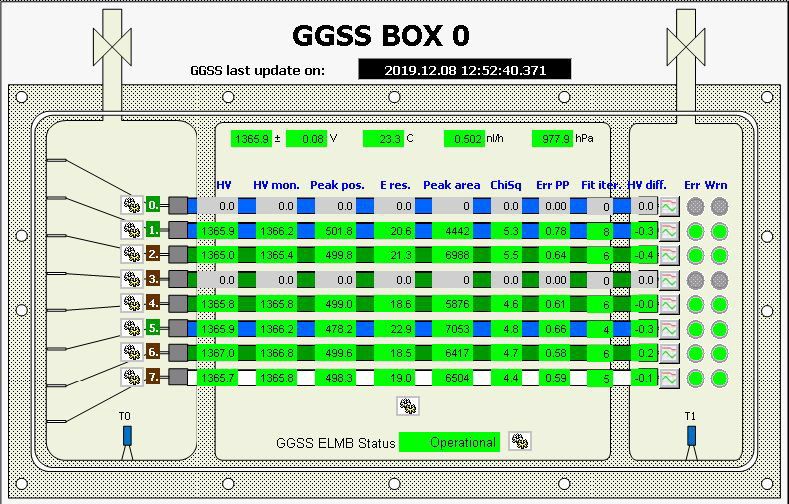
\includegraphics[width=\textwidth]{winccoa_panel.png}
\caption{Fragment przykładowego panelu informacyjno-administracyjnego stworzonego z~wykorzystaniem technologii WinCC OA. Widoczne są m.in.: parametry związane z~pomiarami wykonywanymi za pomocą słomkowych liczników proporcjonalnych (np. \emph{Peak pos.} i~\emph{Peak area}), data ostatniej aktualizacji oraz wskaźniki informujące o~ostrzeżeniach i~błędach.}
\label{fig:winccoa_panel_example}
\end{figure}


Autorzy niniejszego dokumentu nie byli odpowiedzialni za przeprowadzanie prac związanych z~rozwojem oraz utrzymanem systemu WinCC OA funkcjonującego w~ramach infrastruktury CERN. Z~tego też powodu szczegóły jego działania nie zostaną omówione. Istotna, z~punktu widzenia niniejszej pracy, jest natomiast możliwość zastosowania go jako narzędzia ułatwiajacego przeprowadzanie okresowych testów systemu GGSS. Wynika to przede wszystkim z~wygodnej w~użytkowaniu funkcjonalności paneli, pozwalających na monitorowanie działania projektu w~czasie rzeczywistym oraz natychmiastowe wykrywanie wszelkich nieprawidłowości. 


\section{Środowisko docelowe i~ograniczenia}
Charakterystyka środowiska docelowego, w~jakim działa system GGSS, jest z~punktu widzenia niniejszej pracy bardzo istotna, przede wszystkim ze względu na bardzo znaczący związek projektu z~infrastrukturą dostarczaną przez CERN. Stawia to przed autorami szereg ograniczeń dotyczących wersji wykorzystywanych narzędzi, jak również wymusza dodatkowe działania w~przypadku wykonywania pewnych operacji. Do najważniejszych ograniczeń narzucanych przez środowisko docelowe i~specyfikę projektu należą:
\begin{itemize}
    \item dostępna wersja kompilatora języka C++ - w~ramach infrastruktury CERN dostępny jest kompilator \emph{g++ (GCC) 4.8.5}. Wersja ta wspiera w~większości standard C++11, a~zatem funkcjonalności takie jak wyrażenia lambda czy semantyka przenoszenia. Niestety oferowane przez nią wsparcie nie jest pełne - brakuje m.in. poprawnej implementacji biblioteki odpowiedzialnej za przetwarzanie wyrażeń regularnych. Ze względu na wymóg zapewnienia możliwości budowania projektu na maszynie docelowej, ograniczenie to stanowiło znaczące utrudnienie podczas prac nad kodem źródłowym aplikacji wchodzących w~skład systemu.
    \item dostępna wersja narzędzia CMake - na maszynach docelowych dostępna jest wersja \emph{2.8.12.2}, stanowiąca bardzo stare wydanie narzędzia. Oprogramowanie w~znacząco nowszej wersji (tzn. o~numerze wyższym od \emph{3.0}) dostępne jest jedynie na wybranych komputerach wchodzących w~skład infrastruktury CERN, przez co zdecydowano o~pozostaniu przy starym jego wydaniu. Stosowana wersja nie zawiera wielu powszechnie stosowanych współcześnie funkcjonalności oraz charakteryzuje się innym podejściem do zarządzania zależnościami (operacje na poziomie katalogów, uznawane za tzw. \emph{złą praktykę}).
    \item związek projektu z~wersją jądra systemu - jednym z~modułów wchodzących w~skład systemu GGSS jest \emph{ggss-driver}, zawierający sterownik dla wielokanałowego analizatora amplitudy CAEN N957. Istnienie tego modułu wymusza zgodność wersji jądra systemu operacyjnego pomiędzy środowiskiem deweloperskim i~produkcyjnym, co w~konsekwencji prowadzi do komplikacji infrastruktury budowania projektu - konieczne jest stosowanie maszyn wirtualnych oraz narzędzia konteneryzacyjnego Docker podczas procesu budowania komponentu \emph{ggss-driver} (stosowane rozwiązanie opisane zostało przez autorów szczegółowo w~ich pracy inżynierskiej).
    \item ograniczone uprawnienia w~środowisku docelowym - infrastruktura na której uruchamiany jest projekt GGSS jest środowiskiem CERN o~zaostrzonym rygorze. Wszelkie instalowane aplikacje, zmiany w~systemie, bibliotekach, czy też prostych ustawieniach użytkownika muszą być konsultowane z~administratorami systemowymi. Autorzy nie mają możliwości wprowadzania na własną rękę praktycznie żadnych zmian.
    \item możliwość przeprowadzania testów tylko w~określonych momentach prac nad projektem - nad systemami GGSS oraz DCS pracuje wielu ekspertów, testowanie projektu możliwe jest zatem tylko wtedy, gdy nie zakłóca to prac innych osób i~jest fizycznie możliwe (np. gdy nie są wykonywane prace nad warstwą sprzętową systemu). Wymusza to dostosowanie tempa prac w~taki sposób, by jednocześnie testowany był ograniczony, ale znaczący zakres zmian (m.in. by możliwe było szybkie wprowadzenie poprawek w~przypadku wykrycia błędu).
    \item konieczność zachowania kompatybilności wstecznej - zmiany wprowadzane w~systemie nie mogą powodować, że starsze wersje komponentów, z~jakich składa się system GGSS (rys. \ref{fig:high_level_architecture}) staną się niezdatne do użycia, np.: dodanie nowego parametru do pliku konfiguracyjnego nie powinno wykluczać możliwości użycia starszej wersji tegoż pliku oraz starszej wersji oprogramowania. Tego typu ograniczenia obowiązują również w~kontekście danych wymienianych pomiędzy aplikacją GGSS a~systemem kontroli detektora za pomocą protokołu DIM - dane mają odgórnie ustalony, niemożliwy do zmiany format.
\end{itemize}

